\chapter{Debloating Web Applications Using Concolic Execution}
\label{chap:ad}
\section*{Preamble}

So far, in the previous chapters we explored the security gains of debloating web applications. 
We then proposed debloating mechanisms based on dynamic usage traces of users of the web applications to identify unused code sections and remove them through the process of debloating. 
One of the main drawbacks of relying on dynamic traces is the overhead of the instrumentation to collect such code-coverage traces. 
Moreover, dynamic code-coverage as a representation of feature usage for applications lacks generalizability. 
As a result, the correct functionality of debloated web applications would heavily rely on extensive training phase to collect representative usage traces. 
Moreover, slight variations in the behavior of users can result in broken functionality (i.e., functionality that has been removed via debloating). 
This, in part, can be attributed to the properties of line level code-coverage information which is skewed with an over-representation of common and successful code paths (e.g., successful login), and under-representation of unsuccessful and less commonly used yet important features (e.g., forgot password, and error handlers) as evident by the debloated web applications by the ``Less is More''~\cite{azad2019less}.

In this chapter we introduce our approach to address the aforementioned challenges in debloating web applications. 
To this end, we propose the usage of the existing web server access logs to identify web application entry points invoked by the users. 
By focusing on application entry points and abstracting the request parameters and the execution environment (e.g., state of the database), we allow for the exploration of the under-represented paths such as failed login attempts or database errors. 
We perform concolic reachability analysis based on the application's entry points and extract the code-coverage of target web applications in an abstract environment, which allows our results to generalize for \emph{all} user inputs and database states. 
We demonstrate that debloating via concolic execution improves the security of web applications by shrinking the size of their code by an average of 47\% and reducing critical API calls by 55\%, while removing 35-65\% of vulnerabilities for historic CVEs. 
Concolic execution enables us to debloat web applications with comparable security improvements to dynamic debloating schemes without suffering from the runtime overhead, and the need for an extensive training phase. 
Moreover, using concolic execution for debloating, reduces the likelihood of breakage by allowing users to perform all actions reachable from the analyzed entry points.

% After extracting the web application entry points from the web server logs, we perform a reachability analysis by exploring the possible execution paths in the web application through its source code via concolic execution. 
% Concolic execution or concolic testing is a hybrid software verification technique that combines symbolic and concrete execution, by marking symbolic variables as concolic wherever possible~\cite{sen2007concolic}. 
% This enables us to analyze the application in a generic environment where the value of certain request-specific parameters such as session variables, cookies, and HTTP POST parameters are unknown (i.e., symbolic) at the time of analysis. 
% Similarly, we abstract away the database which allows our analysis to identify the reachable code paths and modules that can be invoked based on the HTTP requests from the web server logs regardless of the application database state. 
% At the same time, we incorporate the concrete values for existing information from the web server logs such as HTTP GET parameters and headers such as HTTP REFERER to eliminate concretely unsatisfiable path conditions (e.g., paths that execute if a certain GET parameter is provided). 

% One of the requirements of concolic execution is the instrumentation of the PHP engine to model the result of instructions with symbolic inputs, and exploration of multiple code paths based on symbolic conditions. 
% For that purpose, we build a PHP emulator capable of understanding and emulating \emph{all} PHP opcodes with concrete and symbolic inputs. 
% Moreover, we design a distributed execution environment to allow for the parallel exploration of symbolically satisfiable branches. 

% In the remainder of this chapter, which is replicated from the paper titled ``AnimateDead: Debloating Web Applications Using Concolic Execution'' which is currently under submission, we describe our design for our PHP concolic emulation system called ``\animatedead{}'', and use this system to debloat web applications and report on the improvement of security metrics as a means to quantifying the attack-surface reduction. 

% \pagebreak{}

% \section*{AnimateDead: Debloating Web Applications Using Concolic Execution}

% \subsection*{Abstract}
% Year over year, modern web applications evolve to cater to the needs of many users and support various runtime environments. 
% The ever-growing need to appeal to as many users as possible and the reliance on third-party dependencies comes at the price of code-bloat. 
% Previous research has highlighted the benefits of debloating mechanisms which produce smaller applications, customized to the real needs of their users with significant security improvements. 

% Recognizing the limitations of dynamic and static debloating schemes (including high runtime overhead and lack of accuracy), we propose a hybrid approach based on concolic execution. 
% We developed \animatedead{}, a PHP emulator capable of concolic execution and designed a distributed analysis framework around it. 

% By using the readily available web server logs as application entry points, we perform concolic reachability analysis and extract the code-coverage of target web applications in an abstract environment, which allows our results to generalize for \emph{all} user inputs and database states. 
% We demonstrate that debloating via concolic execution improves the security of web applications by shrinking the size of their code by an average of 47\% and reducing critical API calls by 55\%, while removing 35-65\% of vulnerabilities for historic CVEs. 
% We show that via concolic execution, we can debloat web applications with comparable security improvements of dynamic debloating schemes without suffering from the runtime overhead, and the need for a training phase. 
% Moreover, \animatedead{}-debloated web applications reduce the likelihood of breakage by allowing users to perform all actions reachable from the analyzed entry points.

\section{Introduction}

Web applications and web APIs are the main interface of users with online services. 
WordPress, the blogging platform written in PHP, single-handedly accounts for over 60 million deployments~\cite{wpstatsbuildwith} and 43\% of all websites~\cite{wpstatsw3techs}. 
Therefore, protecting these online platforms against harm by proactively identifying security vulnerabilities and integrating attack-surface reduction mechanisms offers protection to a large user base. 

Modern software aims to be flexible by offering support for various features such as authentication APIs (e.g., built-in authentication and oauth), as well as database adapters (e.g., MySQL vs MongoDB). 
This added flexibility through first party modules and third party dependencies comes at the price of code bloat. 
Code bloat refers to parts of the source code in an application that serve no purpose for their users. 
In the realm of binary applications, researchers focused on identification and removal of unnecessary modules which are often used in code-reuse attacks~\cite{redini2019b, quach2018debloating, 255308}. 

Conversely, code-reuse attacks in web applications only account for a subset of niche vulnerabilities (i.e., object injection attacks). 
In reality, common web application vulnerabilities such as XSS and SQL injection, and those rooted in misconfigurations, reside in reachable parts of the code. 
At the same time, vulnerable functions in web applications often reside in features that are unnecessary for the majority of the users of the applications~\cite{azad2019less}. 
Therefore, web application debloating mechanisms have historically focused on removing live code that is deemed unused under specific workloads. 

Due to the prevalence of dynamic code constructs in web development languages (e.g., PHP, Node.js and Python), end-to-end static analysis is so challenging such that even the state-of-the-art static analysis tools reach an unsupported code structure after analyzing 20 lines of code on average~\cite{altestability}. 
While this limitation is alleviated by localized and context-specific analysis in the realm of vulnerability discovery, debloating requires sound resolution for dynamic code structures (e.g., dynamic file inclusion, functions calls, etc.). 
Failure to resolve dynamic code structures results in removal of necessary features, and therefore, can lead to breakage when interacting with the debloated web applications.

Recognizing this gap between the scalability of dynamic debloating due to runtime instrumentation overhead and accuracy of static analysis due to over-generalizations, we devised a hybrid approach using concolic execution to perform a reachability analysis on target web applications, which we later use to debloat them. 
In this approach, we mark specific sources of information as symbolic (e.g., user controlled values) and the analysis generalizes for all possible values of these parameters. 
The concolic aspect of this analysis consists of transitions of the execution from parameters with symbolic values to concrete values when required. 

We developed \animatedead{}, a distributed analysis system which contains a PHP emulator capable of concolic execution. 
The main contribution of our concolic execution system is its ability to perform end-to-end program analysis. 
Our generic concolic execution engine can be employed for vulnerability assessment, code analysis, and as we discuss in this chapter, for software debloating. 

In this chapter, we focused on using \animatedead{} to perform a module reachability analysis for target web applications given their entry points, and use this information to debloat unused modules. 
This approach benefits from the abstractions of user-provided parameters and an abstract database and network, which results in debloated web applications that retain \emph{all} the code responsible for the exercised entry points from the logs. 
This is in contrast with dynamic debloating schemes that suffer from lack of generalizability, since they only retain the \emph{exact} code paths that were exercised during training, which is biased towards successful actions and overlooks less common yet critical features (e.g., error handlers). 

We show that \animatedead{} is capable of analyzing popular PHP applications (i.e., phpMyAdmin, WordPress, HotCRP, and FluxBB). 
We use the resulting code-coverage of our analysis to debloat web applications and show that by using concolic execution, we can produce debloated web applications that are 25-69\% smaller than their original versions, contain 55\% fewer calls to critical PHP APIs on average, and are exposed to 35-65\% fewer historic CVEs in our dataset, all while maintaining their required functionality. 
In this chapter, we make the following contributions:

\begin{itemize}
    \item We develop and test a feature-complete concolic PHP emulator that supports PHP 5.x and PHP 7.x instructions and is capable of analyzing web applications with abstract inputs and environments.
    \item We use the existing web server log files to extract web application entry points with virtually zero extra overhead, and incorporate them in \animatedead{} to perform a reachability analysis. 
    \item We debloat popular PHP applications and demonstrate the performance of \animatedead{} in improving crucial security metrics such as reducing the size of target web applications and removing historic CVEs. 
    We show that the performance of concolic execution is comparable to dynamic debloating with the added benefits such as offline analysis (no runtime instrumentation overhead) and generalizable debloating (retaining all accessible functions from each entry point).
\end{itemize}
\section{Background}
Program analysis historically incorporates static analysis, dynamic analysis, as well as a hybrid of both. 
While static analysis systems are easier to run at scale, building static analysis tools that support all features within a language is difficult, and even unnecessary in many use cases. 
As a result, it is a common practice to build context-specific static analysis tools by limiting the scope of analysis (e.g., intra-procedural dataflow analysis). 

One of the main limitations of static analysis when it comes to debloating is its inability to perform end-to-end program analysis due to the presence of dynamic code structures. 
An analysis of popular PHP static analysis tools showed that even the state-of-the-art tools fail to analyze more than 20 consecutive instructions before encountering an unsupported code structure~\cite{altestability}. 
% This limitation is exacerbated when such tools are employed for an end-to-end web application analysis which is a requirement for debloating. 
The failure to resolve the dynamic code structures (e.g., file inclusions, dynamic function calls, etc.) results in misjudging the reachability of the required modules. 
Removing such modules causes false positives. 
In other words, the debloated web application will miss files and functions that are required by the users resulting in breakage. 

On the other hand, dynamic debloating schemes such as Less is More (LIM) rely on an extensive training phase during which all the desired features need to be exercised. 
The slightest oversight in the exercised features will result in removal of features that are necessary. 
The authors of LIM build synthetic test cases to model the user behavior. 
An alternative is to perform the training phase on real users by instrumenting live web servers to collect the information about used modules. 
The downside of this approach is the high performance overhead of existing code instrumentation tools such as XDebug, which reportedly, can increase the page load time of web applications by up to 500\%~\cite{azad2019less}. 

\subsection{Symbolic Execution}
\label{sec:background_symbolic}
\begin{listing}[t]
	\begin{minted}[fontsize=\footnotesize, tabsize=2, linenos, startinline]{php}
		$user_name = $_POST['user'];
		if (!isset($username)) {
			$redirect_to = login_url('Username not provided.');
		}
		else {
			$user = get_user_by_login($user_name);
			if (!$user && strpos($user_name, '@') ) {
				$user = get_user_by_email($user_name);
			}
			if ($user) {
				$redirect_to = get_dashboard_url($user->ID);
			}
			else {
				$redirect_to = login_url('Invalid username.');
			}
		}
		wp_safe_redirect($redirect_to);
		exit();
	\end{minted}
	\caption{WordPress login routine. Successful login attempt requires a valid username or email address (line 6 and 8). Conversely, not providing the username or providing a non-existing username results in failed login (line 3 and 14).}
	\label{lst:wordpress_login}
\end{listing}

Symbolic execution is an offline program analysis technique that explores the reachability of different code branches by propagating symbolic values. 
For instance, for web applications, we mark user-provided values as symbolic. 
The symbolic placeholders for the user controlled variables encompass all the possible values for these parameters. 
Throughout the analysis, we collect a set of constraints based on conditional operations and limit the set of feasible values for each symbolic variable. 
Upon encountering a branch with symbolic condition, we fork the execution and explore all feasible branches. 

Listing~\ref{lst:wordpress_login} shows a consice version of the login page of WordPress. 
By running the Selenium scripts from the Less is More dataset, which automate the interactions with common functions of WordPress, we would trigger the successful login via username (first column in Figure~\ref{fig:concolic_coverage}). 
In contrast, symbolic execution explores other paths within the same code leading to the inclusion of functions that handle failed login attempts (line 3, and 14) and login with email address (line 8) as depicted in Figure~\ref{fig:concolic_coverage}. 

\paragraph{Concolic execution:} 
Concolic execution combines concrete and symbolic execution. 
In this scheme, we replace symbolic variables with concrete counterparts depending on the use case. 
For instance, the transition from symbolic values can be used to generate concrete test cases that explore specific parts of an application~\cite{10.1145/1081706.1081750}. 

% \subsection{Challenges}
% %
% While symbolic execution provides a solution to model all possible executions
% of a program, it has its own challenges regarding the execution of real world
% and complex examples.
% %
% The challenges of symbolic execution are classified in four categories: 1)
% Memory, 2) Environment, 3) Space explosion, and 4) Constraint solving.
% %
% In the following, we will describe the challenges that rises for a symbolic
% engine.
% %

% %
% \subsubsection{State Space Explosion}
% %
% One of the main drawback of a symbolic engine is called the state space or path
% explosion problem.
% %
% Depending on the behavior of a symbolic engine, it can fork its execution of
% the program under test during loops, conditional branches, or function calls.
% %
% When a symbolic engine forks the execution of a program, the number of forked
% states can raise exponentially which ends in resource starvation which is
% called state space explosion (i.e., path explosion).
% %
% The major idea behind most solutions for path explosion is to reduce the number
% of states to be explored.
% %
% Each symbolic engine takes on different approach to achieve this.
% %
% Bounding the loop exploration to a limited number of iteration is one approach
% to reduce the number of states to explore.
% %
% An alternate approach is to discard states with un-satisfiable paths from the
% symbolic engines execution queue.
% %
% Prior to executing a forked path, if the constraint solver can prove that a
% logical formula given by the path constraints are not satisfiable, then
% symbolic engine can safely discard the execution.
% %

% %
% Symbolic engines also leverage function or loop summarization to tackle path
% explosion problem.
% %
% A symbolic engine can call a function \texttt{f} multiple times through the
% execution whether at same call-site or different ones.
% %
% Depending on the passed arguments or the call-site, the symbolic engine can
% reuse prior results of invoking the function \texttt{f} for the future
% executions prior to invoking the function.
% %

% %
% Another technique to prevent path explosion is called state merging, where a
% symbolic engine uses constraint solvers to merge multiple states into one in
% order to reduce number of states to be explored.
% %
% State merging has shown to be effective in decreasing the number of path to
% explore.
% %
% However, state merging heavily depends on the constraint solvers of symbolic
% engines which can hamper the performance of symbolic engines.
% %
% Furthermore, symbolic engines utilize different techniques such as taint
% analysis, fuzzing, branch predication, and type checking to prioritize
% different paths to explore.
% %
% Such techniques allow symbolic engines to focus on execution of more promising
% paths without causing path explosion.
% %
% %
% \subsubsection{Memory} 
% %
% Memory is one of the first challenges where a symbolic engine needs to specify
% how it handles complex objects in a programming language including arrays and
% pointers.
% %
% The memory model in a symbolic engine can heavily affect the achieved coverage
% on a program under test.
% %
% One the challenges of handling memory operation is called symbolic memory
% address problem~\cite{SurveySymExec-CSUR18}, where a referenced address in an
% operation in the program is a symbolic expression.
% %

% %
% Symbolic engines can use different level of memory generalization to tackle
% this challenge.
% %
% One can treat all memory addresses as fully symbolic values which is the
% highest level of generalization.
% %
% Symbolic engines take on different techniques in order to implement such
% generalization while accessing symbolic memory addresses such as state forking.
% %
% In state forking, a symbolic engine forks the state of execution on any read or
% write operation on symbolic addresses to consider all possible states of such
% operation.
% %
% An alternate approach is to model all possible memory manipulation in a
% application under test.
% %
% Such level of memory generalization often does not scale to complex
% application, since symbolic execution of a complicated memory operations can
% cause an explosion in number of possible states.
% %

% %
% \subsubsection{Environment}
% %
% The interaction of an application with the environment plays an important rule
% during its execution.
% %
% Most programs are not isolated from interacting wit the environment including
% the operating system such as file system and network.
% %
% As a result, the symbolic engine has to take into account the interaction of
% the application under test with the underlying operating system.
% %

% %
% There are multiple approaches to consider in order to handle environment
% interaction such as concrete execution or abstract modeling of interactions.
% %
% One approach is to perform any OS interaction with concrete arguments.
% %
% Note that the goal of a symbolic engine is to fully explore an application
% execution using symbolic values.
% %
% This solution limits the symbolic engine to fully explore the application since
% the interaction with OS is based on concrete values.
% %
% Another approach is to create an abstract model of the OS interactions such as
% generating symbolic files.
% %
% However, creating an abstract model for the library functions rather than the
% system call in an OS is expensive as the number of functions grows.
% %
% Depending on the application of the symbolic engine, these interactions can be
% handled differently.
% %
% For instance, automatic exploit generation tools models a partial of the system
% environment where an attacker can influence such as file systems and network
% sockets.
% %


% %
% \subsubsection{Constraint Solving}
% %
% There are many techniques that uses constraint solving in order to analyze,
% test, or verify an application.
% %
% For Satisfiability problems (SAT), constraint solvers takes a problem
% represented in a logical formula and determines whether there exist a set of
% boolean values for the symbols that makes the formula true.
% %
% Constraint solving allows the symbolic engine to determine the feasible
% solutions for the executed program, if the feasible solution exists.
% %
% However, constraint solving can be a major bottleneck for the scalability of
% symbolic engine, when it comes down to a complex combination of many
% constraints to solve.
% %
% Constraint solvers use different optimization to tackle the challenge of
% complex constraint such as expression rewriting and constant folding to reduce
% the number of constraints to solve.
% %
% An alternate solution is that constraint solvers use previous constraint
% solutions in order to speed up the constraint solving.
% %

% %
% \subsection{Log files}
% %
% In this subsection we explain how a web server records feedbacks of responding
% to user's requests.
% %
% Web servers such as Apache and Nginx provide a logging mechanism for the
% administrators to collect feedbacks on the activity and the performance of the
% server while responding to requests. \color{red} CITE \color{black}
% %
% The access-logs on a server records all incoming requests that a server
% processes.
% %
% The recorded information on an access-log differs depending on the specified
% format for the web server.
% %
% On a default configuration, when the web server receives a request, it records
% the IP of the machine sending the request, the time stamp, the type of request
% (i.e., \texttt{GET}, ...), the requested file, the response code, and the
% length of the response.
% %
% However, an administrator can customize the format of recorded access-logs
% using the configuration files of the web-server.
% %
% In our system, we extended the access-log formats to include the content of the
% cookies attached to the request.
% %
% Such implementation allows our system to concretize the symbolic value of
% cookies used in a web application on demand. 
% %

% %

\section{System Design} 
\animatedead{} incorporates a PHP emulator which is capable of emulating the execution of PHP code in an environment with abstract entities (e.g., user-provided values, database, network, etc.). 
Figure~\ref{fig:ad_diagram} shows an overview of our system. 
We start by discussing the process to collect the web application entry points. 
Next, we review the design of our emulator and its distributed analysis scheme. 
Then we go over the challenges of PHP symbolic execution such as state space explosion and discuss our approach to addressing them. 
Finally, we use the code-coverage produced by concolic execution of target web applications to perform a module reachability analysis and debloat unused files and functions. 

\begin{figure}[t]
	\centering
	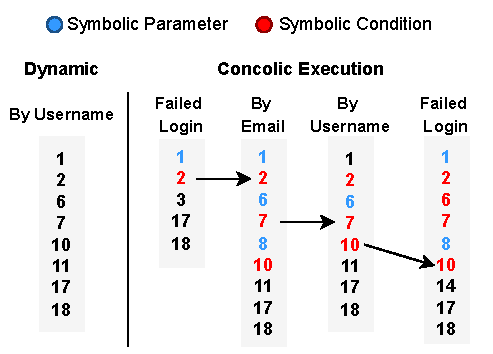
\includegraphics[width=0.5\linewidth]{figures/ad/code_sample_concolic.pdf}
	\caption{Dynamic code-coverage of a successful login attempt vs. symbolic execution of the same entry point. In this sample, user-provided parameters (e.g., \texttt{\$\_POST[\textquotesingle{}user\textquotesingle{}]}) and database operations (e.g., \texttt{get\_user\_by()}) are symbolic. Arrows mark the exploration of new feasible branches as determined by the symbolic engine.}
	\label{fig:concolic_coverage}
\end{figure}

\begin{figure*}[t]
    \centering
    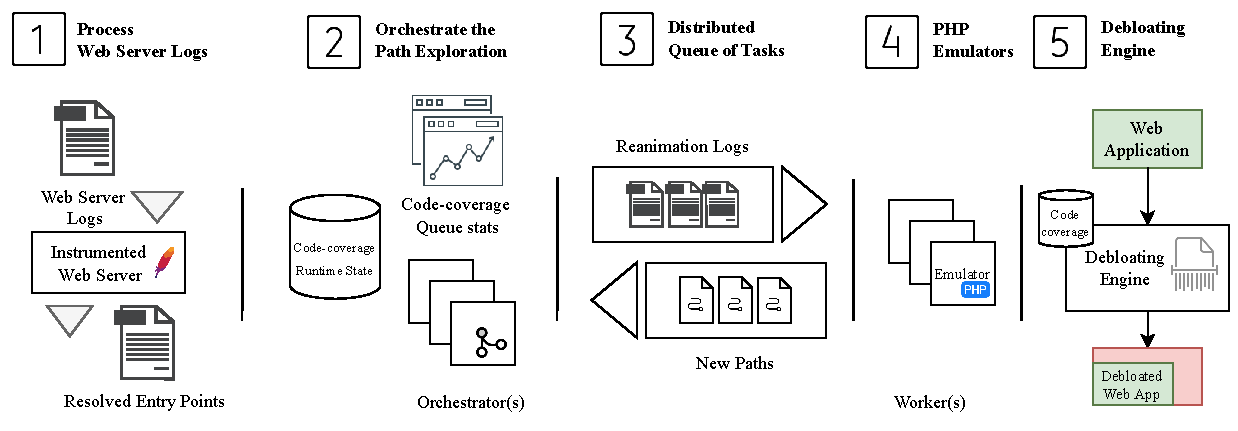
\includegraphics[width=\textwidth]{figures/ad/animatedead_diagram.pdf}
    \caption{Overview of Distributed \animatedead{}. In Stage 1, \animatedead{} analyzes the web server log files to generate unique web application entry points. Orchestrator nodes and workers (Stage 2 and 4) interact over message queues (Stage 3) to identify which paths should be explored by the emulators, \animatedead{} provides a realtime reporting panel that plots the size of the queue and newly identified code-coverage over time. Finally, in Stage 5, the overall code-coverage from concolic execution is incorporated for reachability analysis and unreachable modules from the entry points are debloated. Orchestrators and worker nodes run in container environments and can be scaled up on demand.}
    \label{fig:ad_diagram}
    \vspace{-1em}
\end{figure*}

\subsection{Application Entry Points}
The first step of our analysis consists of collection and processing of web application entry points.  
By using the existing logging mechanism of web servers, \animatedead{} is able to analyze web applications with \emph{no} extra runtime performance overhead. 
At the end of this stage (Step 1 in Figure~\ref{fig:ad_diagram}), we provide the list of PHP scripts and their concrete (e.g., GET parameters) and symbolic parameters (e.g., POST parameters, file uploads, cookies, etc.) to \animatedead{}'s PHP emulators for concolic execution. 

\subsubsection*{Analyzing Web Server Log Files} 
After collecting the web server logs for the target web application, \animatedead{} merges and de-duplicates the entries. 
The level of information provided for each entry point (i.e., concrete inputs) has a direct effect on the time of analysis. 
By shrinking the state space of the analysis via providing more detailed logs, we can reduce the total number of paths and reduce the overall analysis time. 

To that end, we experimented with the default fields of information in web server logs and extended logs. 
To generate extended logs, we use the web server's configuration options to include high level information such as the name (but not the value) of cookies, POST parameters and the file uploads. 
The extra information included in the extended logs limits the concolic execution to only explore paths that rely on the parameters that we have seen previously in the logs. 
Extended logs are particularly helpful for larger web applications such as WordPress and phpMyAdmin where a single entry point is responsible for a diverse list of features depending on the provided parameters. 
For instance, phpMyAdmin uses the same \emph{index.php} entry point combined with the \emph{target} GET parameter to generate the content of the requested pages. 
Providing this parameter to \animatedead{} allows it to only explore code-paths for the desired feature. 

\subsubsection*{Analyzing Log Files With URL Rewriting} 
PHP applications commonly incorporate URL rewriting to provide a user-friendly experience to their visitors and improve the search engine optimization of their website. 
Through this step, the original requested URIs are translated to one of the web application entry points either by the web server (e.g., Apache rewrite module and \texttt{.htaccess} files) or an internal module within the web application (i.e., custom routing modules). 
In the latter case, our PHP emulator resolves this mapping automatically without requiring any further action. 

For web applications using the web server's rewriting feature, the web server transforms the URIs before passing them to the web application. 
For such web applications, \animatedead{} dynamically replays the requests towards its integrated instrumented web server hosting a copy of target web applications and returns the translated entry points. 

\animatedead{} includes an instrumented Apache web server in its docker environment that hooks into every request and returns the translated URIs. 
By intercepting the incoming requests, \animatedead{} takes control of the execution and returns the resolved entry point after the web server applies the rewriting rules.
% Using PHP's \texttt{auto\_prepend\_file} directive, \animatedead{} takes control of the execution while the web server acts upon the original rewriting rules from the source code of target web applications under analysis. 
% This option can be enabled through \animatedead{}'s configuration file. 

\subsection{PHP Emulator}
Concolic execution requires a modified PHP execution environment that can operate based on symbolic parameters. 
We developed a PHP emulator for \animatedead{} that closely represents the PHP engine itself and operates based on the source code of PHP scripts. 
The analysis for each PHP application starts by parsing each entry point (e.g., \emph{index.php}) into it's respective Abstract Syntax Tree (AST) and traversing it. 
Through this traversal, certain PHP instructions will expand the AST during emulation. 
File inclusions, class instantiations, function calls and dynamic code generation routines (e.g., \texttt{eval}) can add new nodes to the AST. 

\animatedead{}'s emulator executes the PHP instructions of the program under analysis and resolves the dynamic code structures to generate a complete AST. 
In practice, resolution of dynamic code structures requires the precise implementation of every language construct and modeling its effects on the state of the emulator (i.e., active namespaces, current object pointers, variable scopes, function calls and return values, etc.). 

In \animatedead{}, beyond modeling the 188 standard PHP opcodes~\cite{popov}, we model the built-in PHP functions that affect the state of the emulator (e.g., loading new classes and defining new constants). 
For the majority of the self-contained PHP built-in functions that do not change the state of the emulator or manipulate the flow of execution such as \texttt{date}, \texttt{print}, \texttt{explode}, \texttt{file\_exists}, etc. we first resolve their arguments and then, invoke the original implementation in the PHP engine. 
For functions that rely on the state of the emulator (e.g., \texttt{class\_exists}, \texttt{define} (defines a new constant), \texttt{reflection APIs} (rely on autoloader and loaded classes and can invoke new code), \texttt{eval}, etc.), we provide our own implementation in the emulator. 
After a careful review of PHP documents and the list of built-in functions used in popular PHP applications, we identified 92 functions that required a custom implementation in our emulator. 

\animatedead{}'s PHP emulator is written in PHP 7.4 and is capable of emulating PHP 5.x and 7.x. 
The emulator imports all the environment variables and predefined constants (e.g., PHP version, default include path, etc.) from an existing web server environment. 
Moreover, analysts using \animatedead{} can override any desired API through the provided configuration file. 

We built our PHP emulator by extending the emulator developed by Naderi et al. called MalMax, which the authors combined with counterfactual execution to uncover the hidden behavior of obfuscated PHP malware~\cite{naderi2019malmax}. 
MalMax was originally built for PHP 5, and did not support symbolic execution. 
We spent over 13 person/months developing and testing our PHP emulator that supports the PHP language features used by popular PHP applications. 

One of our main contributions to MalMax's emulator is the distributed symbolic execution engine. 
Moreover, we added support for integral features of the PHP language to our emulator including the new PHP 7 instructions, object orientation features (e.g., inheritance, interfaces, etc.), closures, anonymous functions, namespaces, and reflection. 
Through this effort, we have doubled the code size of the original PHP emulator of MalMax, and the final \animatedead{} (i.e., emulator plus distributed execution environment) is more than five times the size of the initial emulator. 

\subsection{Handling Symbolic Operations and Logic}
\animatedead{} uses a configurable list of symbolic inputs (i.e., user-provided variables and system APIs). 
In this section, we explain the design details of our concolic emulator, including the type tracking, value set analysis, and the transition from symbolic to concrete values. 



\subsubsection{Concolic Execution}
\label{sec:concolic_translation}
One of the main requirements of a symbolic execution engine is to continue the program's execution with an abstract state of variables. 
At a high level, when dealing with symbolic program variables, PHP instructions such as conditionals would need to explore all the feasible branches when provided with a symbolic condition. 
Similarly, assignment instructions propagate the symbolic values upon their execution.

Our emulator incorporates type tracking to extract the type of symbolic variables even when the actual value is unknown. 
The variable type information is then used to skip the exploration of unsatisfiable branches. 
We model built-in functions that rely on variable types (e.g., \texttt{is\_int}) in the emulator for an accurate execution. 
Similarly, we include our own implementation for instructions that dynamically add new nodes to the AST (i.e., dynamic file inclusion, dynamic function calls, and dynamic object instantiation). 
More specifically, \animatedead{} uses the information available through the execution environment to transform the symbolic variables to their concolic equivalents. 
We will discuss this in more detail later in this section.

An example of this transition is reflected in file export format selection in phpMyAdmin which includes options such as SQL, CSV, Zip, etc. 
Given a symbolic export type in the form of user-controlled variable, \animatedead{} cannot statically determine which of the underlying export plugins should be loaded. 
The \texttt{Plugin\_loader} module within phpMyAdmin performs a series of string operations to sanitize the user input and to transform the selected export format to one of the available plugins on the file-system under the \texttt{libraries/plugins/export/} directory. 
As a result, by following the conditions enforced on the export format variable through execution (e.g., fixed prefix, file extension, and allow-list membership checks), \animatedead{}'s emulator can accurately identify the list of available export plugins in phpMyAdmin. 
Then, the emulator will explore the execution of the underlying entry point using each individual export plugin. 

\paragraph{Type tracking and value set analysis:} 
We have augmented our PHP emulator to track the type of symbolic variables based on known return type of PHP instructions and APIs. 
For instance, casting a symbolic variable to a specific type or invoking built-in functions with known return types (e.g., \texttt{substr} $\rightarrow$ \texttt{string}, or \texttt{isset} $\rightarrow$ \texttt{boolean}) will determine the resulting type of that variable. 
Unfortunately the information about the type of return values from PHP built-in functions is not available through the PHP reflection API. 
Instead, we extracted this information from the PHP documentation and incorporated it in \animatedead{}. 

Moreover, we model regex and string operations (e.g., \texttt{strncmp(\textquotesingle{}pma\textquotesingle{}, \$cookie\_name, 3) \!= 0}) as part of our emulator. 
By doing so, for path conditions that rely on these operations, we track the constraints applied to the underlying variables. 
This way, \animatedead{} can determine non-feasible conditions and refrain from exploring them. 

Lastly, we perform a scope-specific value set analysis. 
Web applications commonly perform allow-list and block-list checks to sanitize user-provided parameters and database sourced values. 
For instance, phpMyAdmin performs the following allow-list check to sanitize and validate the user-provided viewing mode in the reporting tabs: \texttt{in\_array(\$\_REQUEST[\textquotesingle{}viewing\_mode\textquotesingle{}], array(\textquotesingle{}server\textquotesingle{}, \textquotesingle{}db\textquotesingle{}, \textquotesingle{}table\textquotesingle{})}. 
When exploring paths that satisfy this symbolic condition, \animatedead{} limits the possible values of the symbolic \texttt{\textquotesingle{}viewing\_mode\textquotesingle{}} parameter to the values in the corresponding array (i.e., \texttt{\textquotesingle{}server\textquotesingle{}}, \texttt{\textquotesingle{}db\textquotesingle{}}, or \texttt{\textquotesingle{}table\textquotesingle{}}). 
This feature helps reduce the total number of explored branches and also aids the concolic engine when transitioning from symbolic values to their concrete counterparts. 


\paragraph{Transition from symbolic to concrete values:} 
The main benefit of symbolic execution is that each symbolic value represents all the possible values for that variable. 
As a result, it is beneficial to continue the execution with symbolic values. 
However, there exists scenarios in which \animatedead{} cannot continue executing the target application symbolically. 

Whenever our emulator reaches a PHP instruction that can change the structure of the AST by adding new files or calling new functions, \animatedead{} must replace the symbolic inputs of that API with its concrete counterparts. 
Examples of the APIs that add new nodes to the AST are file inclusion APIs (e.g., \texttt{include \$var}), class instantiations and static function calls that trigger the PHP autoloader (e.g., \texttt{new \$var} or \texttt{\$var::static\_function()}), reflection APIs, variable function calls (\texttt{\$var()}), APIs accepting a callback (e.g., \texttt{call\_user\_func(\$var)} and \texttt{preg\_replace\_callback(/regex/, \$var)}). 

In any of the aforementioned cases, \animatedead{} will rely on the information available from the execution environment to transition to concrete values. 
Most commonly, this step would consist of using the type information to determine the class type (for object instantiation), mapping the string operations to the file system or using the information from the value set analysis to determine the candidate values for each symbolic variable. 

Whenever the emulator faces more than one concrete option for a symbolic variable, it will create a new task including the code-coverage of the current execution and information about the concrete values for the target variable and add this task to the queue for future concolic execution (bottom queue in Step 3 in Figure~\ref{fig:ad_diagram}). 
Orchestrators process the code-coverage of each execution. 
Discovery of new code-coverage increases the priority of descendant paths of the current execution. 
\animatedead{} provides a configuration option to limit the total number of concrete values added from each point in the web application. 
% Based on our observations on PHP applications and their coding patterns, we set this limit to 20. 

In the scenario where symbolic execution cannot provide any information about the value of variables used in dynamic file inclusions or function calls, \animatedead{} would not be able to correctly determine the target files and functions to execute next. 
While in theory such code structures exist, and they could lead to false positives, in practice, we did not observe \emph{any} of them. 
An unbound symbolic file inclusion or function call may be rooted in non-sanitized user controlled variables or parameters coming from the database. 
In both scenarios, this could signal the presence of a first or second order injection style vulnerability and requires further attention. 
We incorporated safety checks within \animatedead{} to prevent the inclusion of an uncontrollably large number files or functions when the symbolic parameter is unbound and instead, we alert the analysts. 

\subsubsection{Emulation Replay} 

Throughout the analysis of PHP scripts, for every branch with symbolic condition, \animatedead{} explores all feasible paths. 
Similarly, when transitioning from symbolic to concrete values, multiple execution states are added to the queue. 
Upon facing more than one path to explore, the emulator produces a log called ``reanimation log'' which marks the currently explored branches and lists the next symbolic branch that should be explored. 
Using the reanimation logs, \animatedead{} instructs the emulator in worker nodes to replay the same execution and explore new branches within the code (top queue in Step 3 of Figure~\ref{fig:ad_diagram}). 


\subsubsection{Sources of Symbolic Information} 

In our analysis, we marked HTTP requests and their parameters, database APIs, and network APIs as symbolic. 
Therefore, the result of the analysis is a generalization over \emph{all} the possible values for the parameters present in the web server logs for the application under analysis. 
In our study we opted to run our analyses with an abstract application database. 
This way, our analysis generalizes for \emph{all} deployments of the web applications with any state of the database (i.e., successful and failed connections, empty and non-empty tables, etc.). 
Lastly, we mark network request responses as symbolic to account for successful and failed requests (e.g., checking for updates).

For HTTP requests, we instruct \animatedead{} that HTTP Cookies, Session variables, and File upload and POST parameters (For POST requests) are symbolic. 
This is based on the intuition that web servers will log HTTP GET request parameters and their values by default (i.e., URL query strings) but the value of cookies, session variables, and POST parameters are not included in neither default nor extended logs as they can include sensitive information. 
For database abstraction, we referred to the PHP language documents to extract the list of database APIs for popular database backends~\cite{phpdatabaseapis} and marked them as sources of symbolic information. 
Lastly, we marked PHP cURL APIs as symbolic to abstract the effect of network requests. 

\paragraph{Handling file uploads and file modifications/deletions:} 
PHP engine stores information about the uploaded files in the \texttt{\$\_FILES} super global variable. 
Each entry in this array corresponds to one of the user-uploaded files and contains information such as name, mime-type, temporary name (i.e., temporary file storage under /tmp/php/ directory by default), error (error code or 0 if successful), and size (upload size in bytes). 

For entry points with file uploads, \animatedead{} populates this super global variable with symbolic entries including successful and failed file uploads. 
Moreover, file operation APIs (e.g., \texttt{fopen, file\_get\_contents}, etc.) are modeled inside our emulator to handle symbolic file uploads. 
That is, opening a symbolic file will return a file with symbolic content. 
All web applications in our dataset perform file upload operations and our tests invoke the underlying entry points. 

When running multiple concolic execution workers in parallel, we isolate the changes they make to the file system to prevent side effects on other executions. 
\animatedead{} intercepts the APIs used to modify (e.g., \texttt{file\_put\_contents}) or remove files (e.g., \texttt{unlink}) and changes made through these APIs are only visible to the currently running execution. 
Therefore, file system modifications from one worker do not affect future executions and other workers. 

\subsection{Distributed Concolic Execution} 

Throughout the analysis of target applications, \animatedead{} will explore millions of different paths. 
To scale up the analysis, we designed a distributed environment with various worker processes running our PHP emulator. 
In this setup, we designate a group of orchestrator nodes responsible for the code-coverage analysis of the workers and prioritization of next paths to explore (Step 2 in Figure~\ref{fig:ad_diagram}). 
Orchestrators compare the code-coverage of current execution with the previously explored code and prioritize the analysis of unexplored branches, specifically the descendants of executions that resulted in the exploration of new parts of the code-base. 

\subsubsection{Path Prioritization}

We try to address the problem of state space explosion from two directions:
\begin{itemize}
    \item Eliminating unsatisfiable paths and limiting the total number of explored paths.
    \item Prioritizing paths based on their likelihood to explore unique parts of the codebase.
\end{itemize}

\paragraph{Reducing the total number of feasible paths:} 
Through close inspection of the structure of popular web applications, we identified that the majority of symbolic conditions check for presence or absence of user-provided parameters. 
These parameters usually dictate the main control flow of the entry points (e.g., providing username and password in a login request). 

Given the list of user controlled parameters (i.e., Post, Cookie, and Session variables) in phpMyAdmin, we analyzed the constraints for symbolic conditions. 
Overall, we identified that on average, 72\% of symbolic conditions only check for presence or absence of such parameters through the \texttt{isset} and \texttt{empty} built-in functions. 

Based on this observation, we decided to include the name (and not the value) of these parameters in the extended web server logs. 
This way, we will have the list of provided parameters by the users for POST requests and file uploads, thereby, significantly reducing the number of symbolic paths to be explored by \animatedead{}. 
% Moreover, we use the type tracking of \animatedead{} to eliminate the exploration of unsatisfiable branches in conditions on symbolic variables with a known type. 

\paragraph{Efficient path selection:} 
The exponential growth in the total number of paths in the application under analysis requires an effective path selection strategy. 
Symbolic execution engines employ problem-specific heuristics to analyze paths that are more likely to yield the desired results first. 
In the current setup, we opted to optimize paths to maximize code-coverage that is reachable from each entry point. 
\animatedead{} implements two path prioritization algorithms:

\begin{itemize}
    \item \textbf{DFS:} Using the depth-first-search algorithm, emulator worker processes will choose the last symbolic branch and flip its last symbolic condition to explore the new paths. This is the most straightforward approach that lacks any optimization for maximizing the explored code-coverage. 
    This method would result in the assignment of the same priority to all paths.
    \item \textbf{Branch-coverage guided prioritization:} In this setup, orchestrator nodes keep track of the branch coverage across all workers and prioritize paths that will explore the unseen branches. 
    For branches that have never been explored before, we set the priority to the maximum of 100. 
    After covering all the unique branches at least once, we calculate the priority by adding the total number of new lines discovered by each execution to 20\% of the priority of the parent branch for a maximum of 100. 
    This way, we focus on expanding the coverage in the vicinity of the recently discovered code, while gradually reducing the effect of the priority inherited from the parent execution to prevent the analysis from getting stuck in repetitive code structures. 
\end{itemize}

\begin{figure}[t]
    \centering
    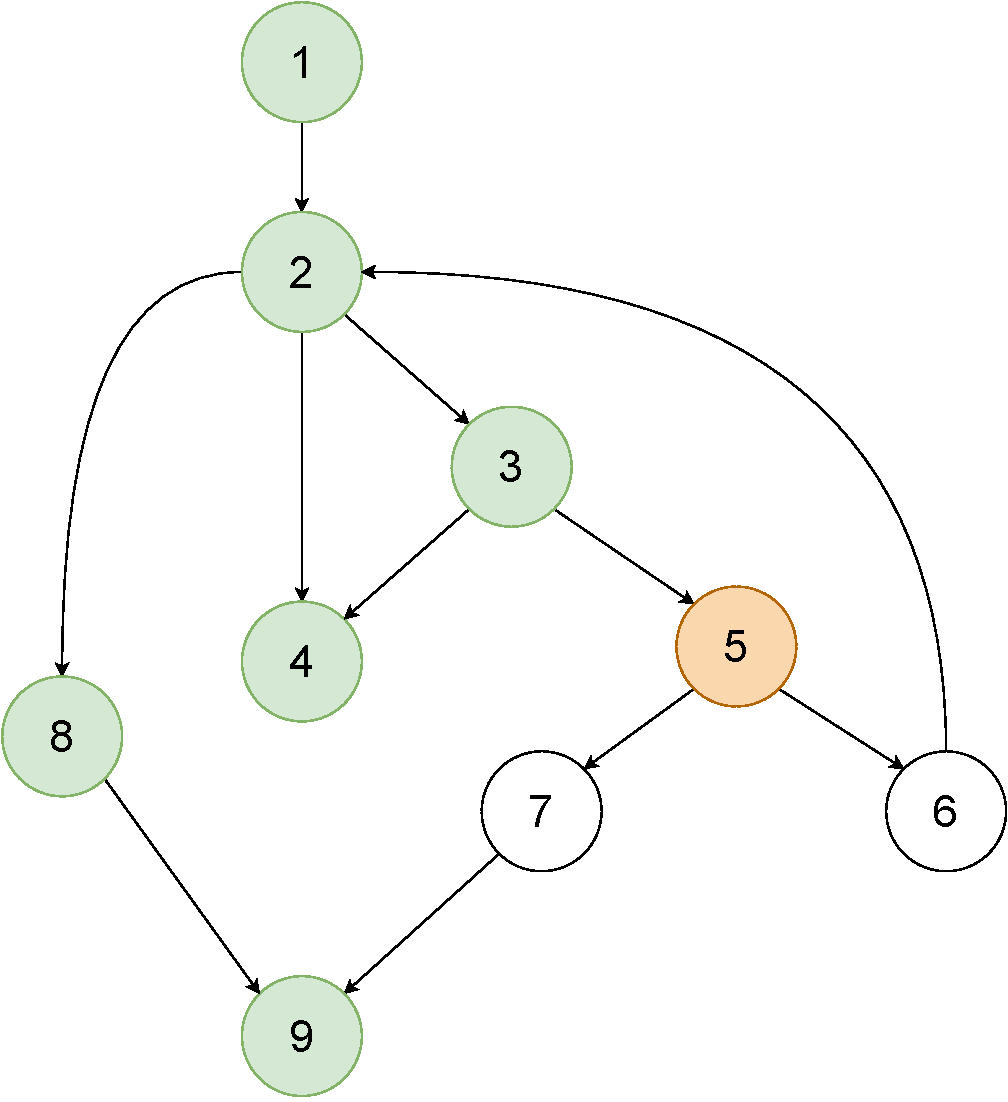
\includegraphics[width=0.3\linewidth]{figures/ad/AD_Path_Prio_CFG.pdf}
    \caption{Control flow graph example for path prioritization}
    \label{fig:cfg_pathprioritization}
\end{figure}

In the sample control flow graph in Figure~\ref{fig:cfg_pathprioritization}, assuming that all branches are symbolic, and the green nodes have been explored, once the two branches from node 3 are identified, the exploration of the branch towards node 5 receives the maximum priority of 100, as it has never been explored before. 
Moreover, immediate children of node 5 also inherit 20\% of the priority of their parent (i.e., 20) as they are the descendants of a newly discovered node. 

We store the reanimation logs on a priority queue, and as a result, workers will explore branches with a higher score first. 
We will compare and contrast the performance of DFS vs. Branch coverage path prioritization methods in Section~\ref{sec:path_priority}. 

\subsection{Debloating the Web Applications}
\animatedead{} produces the code-coverage information by merging the individual code-coverage from each execution of its workers. 
These results are analogous to the dynamic code-coverage used for debloating by the prior work. 
% The main benefit of this approach is the ability to perform an offline analysis based on web server logs.  
After generating the code-coverage for each web application, \animatedead{}'s debloating engine (Step 5 in Figure~\ref{fig:ad_diagram}) performs a reachability analysis and removes unused modules (i.e., files and functions) from the source code of web applications. 
We report the size reduction and security gains of debloating web applications via concolic execution and contrast the performance of this debloating scheme with the dynamic debloating of Less is More in Section~\ref{sec:results}. 

\subsection{Correctness Tests During Development}

During the initial stages of the development of our emulator, we started extracting the list of all PHP instructions from the PHP parser and provided an implementation of their logic in our emulator. 
Next, we analyzed the source code of popular PHP applications such as WordPress and phpMyAdmin to extract samples of interactions with symbolic variables (i.e., database queries, code handling HTTP requests, etc.).  

\paragraph{Unit Tests:} Based on the code snippets extracted from these applications, we created a total of 199 unit tests. 
We also included 19 unit tests provided by MalMax in our test suite~\cite{naderi2019malmax}. 

\paragraph{Functional Tests:} To complement the unit tests, we ran the Selenium scripts published as part of ``Less is More''~\cite{azad2019less} on debloated web applications. 
For the web applications in our dataset that are not part of LIM's dataset, we assembled a list of tasks exercising the main functionality of these web applications. 
For HotCRP, our scripts automate the setup of a conference and its deadline, user creation, submission of papers, and submitting reviews. 
For FluxBB, we automate user creation, posting new topics and changing user preferences. 
The extensive list of tasks that we automated with Selenium scripts is available in the Appendix. 

We then compared the list of invoked files and functions in response to requests towards debloated web applications and through iterative debugging we identified and addressed the implementation bugs that would prevent \animatedead{} from invoking the same modules as listed in the dynamic code-coverage traces. 
\section{Evaluation and Results}
\label{sec:results}

\begin{table}[]
    \caption{Number of automated daily requests towards web applications compared to the number of unique entry points.}
    \centering
    \begin{tabular}{|l|l|l|}
    \hline
    \textbf{Web Application} & \textbf{Requests/Day} & \textbf{Unique Endpoints} \\ \hline
    WordPress                & 558,576               & 152 (99.97\% $\blacktriangledown$)             \\ \hline
    phpMyAdmin               & 491,400               & 107 (99.98\% $\blacktriangledown$)             \\ \hline
    HotCRP                   & 175,848                 & 32 (99.98\% $\blacktriangledown$)              \\ \hline
    FluxBB                   & 63,624                & 17 (99.97\% $\blacktriangledown$)              \\ \hline
    \end{tabular}
    \label{tab:logreduction}
\end{table}

In this section, we employ \animatedead{} to debloat web applications. 
We start by collecting the list of entry points exercised while using popular web applications. 
We then configure \animatedead{} to explore feasible paths from those entry points. 
The result of this step is a list of exercised modules in target web applications. 
These modules are reachable from the list of entry points. 
Then, by removing the unused modules, we produce debloated web applications. 
In the remainder of this section, unless mentioned otherwise, we discuss the results of function debloating (i.e., removing functions with no callers) as it strictly outperforms file debloating.

Debloating based on concolic execution in \animatedead{} has multiple benefits over the previously explored dynamic debloating schemes that rely on runtime tracing to collect code-coverage information from users:

\begin{itemize}
    \item By relying on existing logging mechanism of web servers, we can collect usage traces for long periods of time for web applications with a large user base with small overhead.
    \item By analyzing each entry point in an abstract state (i.e., abstract request parameters, database, and network requests), the resulting code-coverage incorporates the functionality for all actions that are possible through each entry point and all possible database and network responses (i.e., including successful and failure cases), resulting in robust debloated applications (Section~\ref{sec:automated_random_testing}). 
\end{itemize}

\subsection{Experimental Setup}

In our evaluation, we focus on four popular web applications with different size and functionality. 
Our dataset includes phpMyAdmin 4.7 (database administration), WordPress 4.6.22 (content management system), HotCRP 3.0 (submission management), and FluxBB 1.5.11 (online forum platform). 

We run our analysis using 20 worker nodes (running \animatedead{}'s PHP emulator), and 5 orchestrators running inside Docker on an Ubuntu 22.04 LTS host with 20 CPU cores and 32GB of memory. 
For each web application, we follow their installation steps to generate the configuration files. 
This step is necessary as \emph{all} web applications in our dataset verify the presence of configuration files (e.g., \texttt{wp-config.php} for WordPress) and redirect user requests to the installation page if the post-installation files are absent from the file system. 

We configured concolic execution campaigns with the threshold of 24 hours, though in practice, the majority of entry points converge to their maximum code-coverage in less than one hour. 
Analysts can observe the progress made by \animatedead{} through the reporting panel and decide to terminate the analysis when \animatedead{} stops identifying new code-coverage or the queue becomes empty (i.e., all paths for an entry point are explored). 

\begin{figure*}[t]
    \centering
    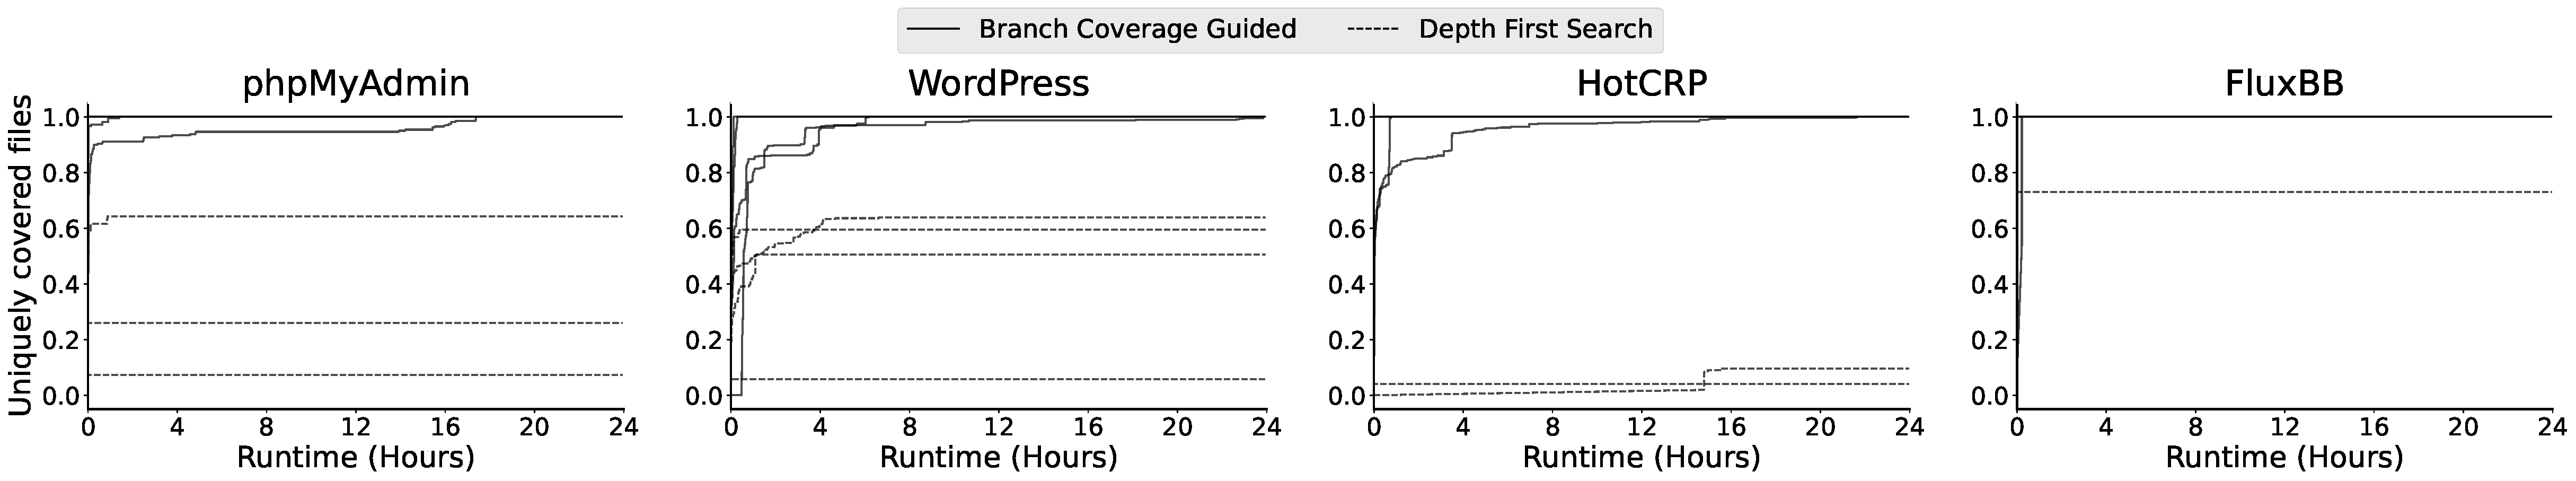
\includegraphics[width=\textwidth]{figures/ad/execution_convergence.pdf}
    \caption{Unique files discovered over time using DFS and Branch coverage guided path prioritization. Branch coverage approach results in a higher number of discovered files while DFS gets stuck in the same parts of the code.}
    \label{fig:execution_convergence}
\end{figure*}

\subsubsection*{Data Collection} 
To compare the debloating performance of \animatedead{} with prior work and to generate baseline code-coverage information for each entry point, we rely on the automated tests provided by the ``Less is More''~\cite{azad2019less}. 

We run the Selenium scripts from Less is More and the ones we built for HotCRP and FluxBB and collect the web server logs along with the dynamic code-coverage information from the Less is More framework. 
The code-coverage information for our web applications serves as the baseline code-coverage (i.e., dynamic code-coverage) for the remainder of our evaluation. 

We expect the resulting code-coverage of \animatedead{} to be a superset of the dynamic code-coverage information. 
Any file or function covered in the dynamic code-coverage that is missed by \animatedead{} would signify a false positive (i.e., removal of a feature that is required by users). 

\subsubsection*{Data Cleaning and Summarization} 
It is common for popular entry points (e.g., \texttt{index.php}) of web applications to receive a large number of requests. 
To prevent our tool from performing the same analysis multiple times unnecessarily, we only retain unique entry points and parameters from the web server logs. 

In the initial stages of the analysis, \animatedead{} removes duplicate log entries. 
Since we analyze the application with an abstract database, different values for the same parameters will have a similar effect (e.g., \texttt{?page\_id=1} or {\texttt{2}). 
This deduplication also shrinks the total number of entry points significantly. 
Table~\ref{tab:logreduction} lists the total number of log entry points produced over a 24 hour period by running the automated tests (Selenium, and crawler) repeatedly (simulating different users of a web application exercising the same functionality), compared to the final number of unique entries used by \animatedead{} for analysis. 
Across all web applications in our dataset, we observe a reduction of over 99.9\% in the number of unique entries to be analyzed. 
Moreover, web applications with a smaller code-base (i.e., FluxBB and HotCRP) produce fewer unique entry points. 

\subsection{Generating the Code-coverage}

We take the logs for each entry point in the web applications in our dataset and run them in \animatedead{} until either all paths are exhausted or a timeout of 24 hours is reached. 
\animatedead{} produces the code-coverage information for each execution in a separate log file. 
After merging the code-coverage of the explored paths from all entry points, we perform a module reachability analysis at the file and function level and debloat unreachable files and functions. 

\subsubsection{Efficient Path Selection}
\label{sec:path_priority}
Concolic execution generates an exponentially growing number of paths to be explored in target applications. 
This number grows based on the number of symbolic conditions in the target applications, for which \animatedead{} would need to explore the execution of all feasible branches. 
Concretely, \emph{N} consecutive symbolic branches would produce 2\textsuperscript{N} distinct paths. 

The prevalence of symbolic conditions and the total analysis time of each entry point directly affect the size of the queue which contains the future paths to be explored. 
Figure~\ref{fig:execution_convergence} depicts the unique files covered over time for a subset of entry points in each web application in our dataset during 24 hours of runtime. 

We ranked the time it takes for \animatedead{} to converge to the maximum file coverage for all application entry points. 
We then picked one entry point from each quantile for a total of four entries for each web application and path prioritization algorithm. 
For instance for WordPress, we plot ``admin-ajax'', ``customize'', ``index'', and ``login''  entry points sorted from most to least time to converge. 

Solid lines in Figure~\ref{fig:execution_convergence} represent the ratio of maximum covered files for each entry point when configuring \animatedead{} with Branch coverage guided path prioritization and dotted lines represent the runtime of the same entry points with DFS. 

For smaller applications such as FluxBB, the code-coverage converges in less than 10 minutes. 
For \emph{index.php} entry point of FluxBB, DFS fails to identify \emph{all} reachable files and is stuck in a repetitive code structure. 
For web applications with a modular architecture in which a larger number of PHP files are invoked to respond to each request, concolic execution requires a longer time to converge. 
This effect is visible for \emph{server\_import.php} entry point which explores code-paths for various export formats and takes 17 hours and 23 minutes to converge to its maximal code-coverage. 
Similarly, for WordPress, while the majority of entry points converge in the first few hours, certain entry points (e.g., such as \emph{admin-ajax.php} and \emph{customize.php}) take between 6 and 20 hours to converge. 

Across all web applications, we observe that branch coverage guided prioritization outperforms DFS in terms of the overall code-coverage. 
In practice, using the DFS algorithm leads to missing code-coverage (mainly due to investing the majority of execution time in the same subgraphs of the AST) which results in false positives after debloating. 

% \subsubsection{Correctness of Code-coverage}

% The validity of the debloated web applications by \animatedead{} relies upon the correctness of the resulting aggregate code-coverage for all application entry points. 
% There are two threats to the validity of this coverage:

% \begin{itemize}
%     \item Digression in the behavior of the PHP emulator compared to original PHP engine due to implementation flaws.
%     \item Feasible execution paths not being prioritized over previously explored paths, which results in missing code-coverage, due to suboptimal path prioritization.
% \end{itemize}

% After running the analysis of the entry points in \animatedead{} and collecting the overall code-coverage, we perform a reachability analysis and remove unused files and functions from the source code.
% This step provides us with the debloated web applications.

% In the absence of a ground truth dataset including all the reachable code from a given set of entry points for each web application, we rely on automated and random testing. 
% To empirically evaluate the correctness of \animatedead{} we devise two set of tests. 
% For each debloated web application, first, we replay the same tests used to collect the entry points and generate the dynamic code-coverage to make sure the debloated web applications did not lose any of their required functionality after debloating. 
% Second, we fuzz each entry point using an automated crawler. 
% In the case of correct debloating, the fuzzer would not trigger any debloated code while operating on the same entry points.

\subsection{Debloating Metrics}
We report the effectiveness of our debloating scheme through various source code and security metrics. 
These metrics are proxy variables to quantify the security improvements of debloated web applications. 

\subsubsection*{Logical Lines of Code (LLOC) Reduction} 
The reduction in the overall size of the code-base of an application has a direct correlation with the number of bugs present in it~\cite{mcconnell2004code}. 
Based on this intuition, shrinking the size of an application's code-base by removing unnecessary features reduces its attack surface and potential vulnerabilities. 
To measure this, we report the size of applications in our dataset before and after debloating in terms of logical lines of code (LLOC). 

\begin{table}[]
    \caption{LLOC reduction results of \animatedead{} compared to Less is More. Percentages represent the code reduction ratio.}
    \label{tab:lloc_reduction}
    \centering
    \begin{adjustbox}{max width=\columnwidth}
        \begin{tabular}{|l|l|l|l|}
        \hline
        \textbf{Web Application} & \textbf{Original} & \textbf{AnimateDead} & \textbf{LIM}  \\ \hline
        phpMyAdmin               & 112,220           & 35,162 (69\%)        & 26,094 (77\%) \\ \hline
        WordPress                & 73,201            & 39,529 (46\%)        & 36,738 (50\%) \\ \hline
        HotCRP                   & 40,898            & 30,814 (25\%)        & 24,407 (40\%) \\ \hline
        FluxBB                   & 6,683             & 3,550 (47\%)         & 3,141 (53\%)  \\ \hline
        \end{tabular}
    \end{adjustbox}
\end{table}

Table~\ref{tab:lloc_reduction} lists the size of web applications by \animatedead{} and Less is More (LIM). 
In this setup, \animatedead{} is performing concolic exploration of the same entry points as invoked by dynamic tests for LIM. 
As a result, the code-coverage produced by \animatedead{} is a superset of LIM. 
By looking at Table~\ref{tab:lloc_reduction}, we observe that for most web applications, debloating via concolic execution provides a size reduction comparable to the dynamic debloating. 

% Upon closer inspection of the files kept by \animatedead{} and removed by LIM, it is evident that dynamic debloating only kept the specific code path invoked via training while \animatedead{} kept the code responsible for the functionality that was reachable from each entry point including the error handlers and various code paths that lead to the invocation of the same feature. 

Upon closer inspection of the code that is only covered by \animatedead{} we identified features that were never exercised by Selenium tests but were reachable from the entry points. 
This enhances the usability of debloated web applications by \animatedead{} and reduces the likelihood of users invoking a removed function, which is a major drawback for dynamic debloating systems. 
For instance, we identified that the ``Forgot password'' functionality, reachable from the login entry point of WordPress was never invoked during the dynamic tests, and therefore, was removed by LIM. 
We verified that \animatedead{} keeps this functionality in WordPress, and as a result, allows users to use ``forgot password'' functionality even after debloating. 

\paragraph{Key point:} 
By incorporating concolic execution to explore the feasible program execution paths, \animatedead{} is able to generate the code-coverage of target web applications, reachable from their entry points. 
Using this code-coverage for reachability, allows us to produce debloated web applications that allow their users to perform all actions that are reachable from the previously invoked entry points, thus, reducing the likelihood of interacting with a debloated feature. 

\subsubsection*{Critical API Call Reduction}

\begin{figure}[t]
    \centering
    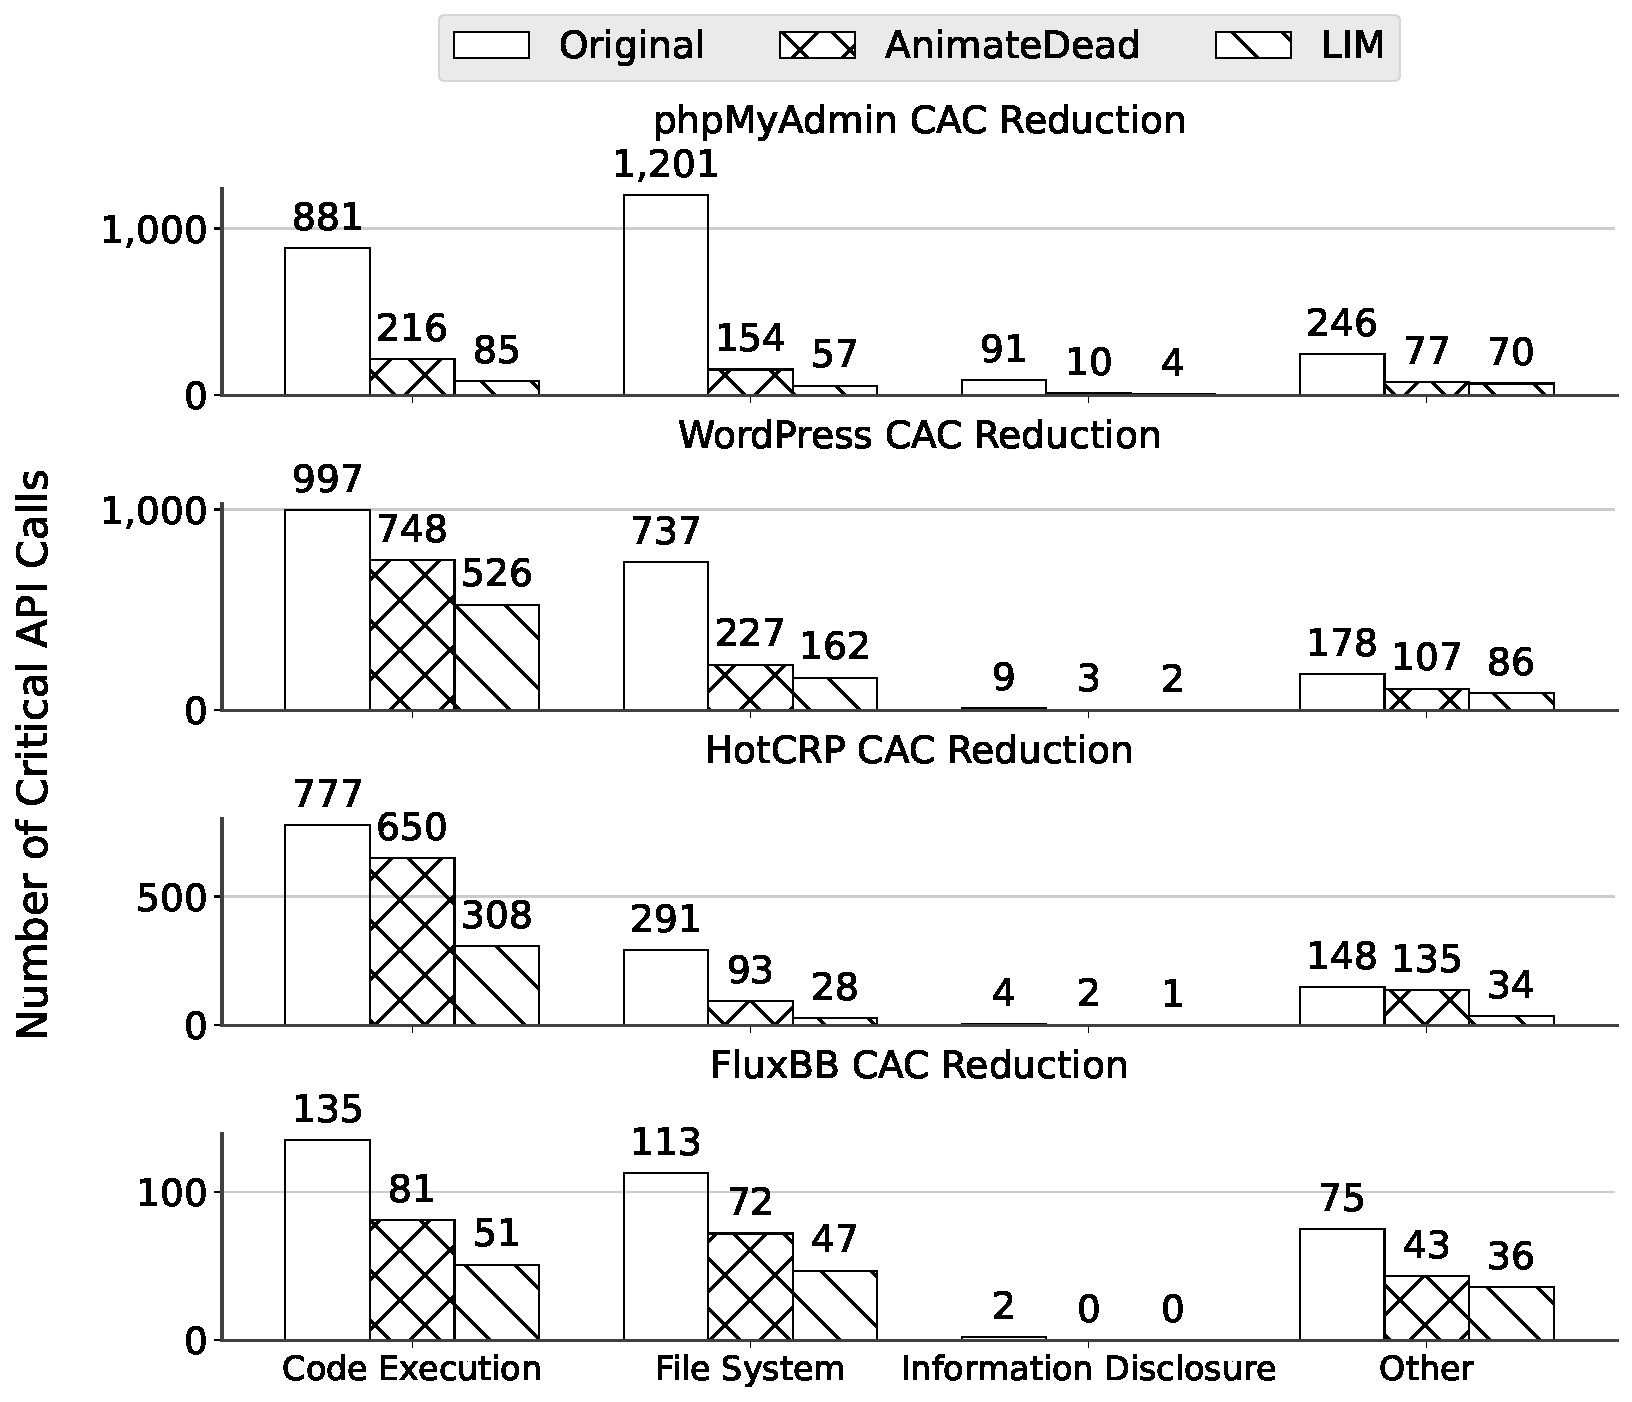
\includegraphics[width=0.9\columnwidth]{figures/ad/cac_reduction_bw.pdf}
    \caption{Reduction of Critical API Calls.}
    \label{fig:cac_reduction}
\end{figure}

The PHP engine interacts with its execution environment through a set of internal APIs. 
These APIs enable web applications to interact with the file system, network or even the database. 
Similar to system calls in binary applications, abuse of Critical PHP APIs (e.g., \texttt{eval}) is closely related to the amount of damage an attacker can do. 
Previous work in the area of exploit prevention and debloating has emphasized the importance of protecting critical APIs~\cite{Mishra2018, pappas2012kbouncer, fratric2012ropguard, bulekov2021saphire}. 

We use the list of 205 critical APIs used by RIPS to perform taint analysis on PHP applications for vulnerability discovery~\cite{dahse2010rips}. 
We report the removal of these APIs after debloating. 
For phpMyAdmin, we observe that \animatedead{} removes 75\% of code execution API calls, compared to 90\% reduction of Less is More. 
For other applications in our dataset, this reduction of critical API calls ranges from 10\% to 89\% for \animatedead{} and 50\% to 96\% for Less is More. 
As demonstrated in Figure~\ref{fig:cac_reduction}, debloating based on concolic execution of entry points results in a considerable reduction in critical API calls compared to the original applications, across all categories of critical APIs. 

\subsubsection*{CVE Reduction}
Orthogonal to size reduction, we measure the performance of debloating in removing historic vulnerabilities in the source code of an application. 
To that end, for web applications present on public CVE databases (phpMyAdmin and WordPress), we reuse the CVE to source code mapping information available in the prior work~\cite{azad2019less}.

Table~\ref{tab:cve_reduction} lists the removal of CVEs after debloating. 
For both web applications, file debloating of \animatedead{} and LIM remove the same number of CVEs. 
Similarly, for WordPress, function debloating of \animatedead{} and LIM retain seven CVEs. 
For phpMyAdmin, function debloating results show that \animatedead{}'s debloating retains three CVEs more than LIM. 

We analyzed the three extra CVEs. 
For the first vulnerability (CVE-2016-5703), LIM retains multiple call sites for the vulnerable function, none of which were invoked during the dynamic tests. 
Since the path conditions for these call sites rely on database values (i.e., symbolic), \animatedead{} correctly retains the vulnerable function to preserve the correct functionality. 
Second vulnerability (CVE-2016-6633) resides in the ``import'' page of phpMyAdmin. 
Selenium tests only import SQL files while phpMyAdmin supports seven formats (e.g., zip, CSV, XML). 
Since the uploaded file format is selected by the user and is therefore symbolic, \animatedead{} retains other import formats including the one with the vulnerability. 
Lastly, we analyzed CVE-2016-6619 which resides in ``recent favorite tables'' feature, if the users request the list of recent tables without having selected any tables before, the vulnerable function would be invoked. 

The performance of \animatedead{} and LIM in the removal of CVEs for WordPress is identical. 
For the three CVEs that were removed only by LIM, we analyzed the source code of phpMyAdmin and identified that in all cases, there exists at least one symbolic code path (based on user-controlled parameters or database values) that can call the vulnerable functions, and therefore, \animatedead{} correctly retained the CVEs to preserve the correct functionality in the debloated web application. 


\subsubsection*{Removal of Object Injection Gadgets}
Improper use of deserialization APIs in PHP can lead to object injection vulnerabilities. 
This vulnerability allows attackers to build a chain of function calls through existing classes in the vulnerable web applications--known as gadget chains--to mount exploits such as SQL injection, arbitrary file write, and even remote code execution. 

Removal of gadget chains via debloating protects web applications and complicates the exploitation of object injection vulnerabilities. 
We use PHPGGC, a public repository that tracks the known gadget chains in popular web applications and third-party packages~\cite{PHPGGC}, to identify gadgets for phpMyAdmin and its third-party packages as well as WordPress. 
Their dataset does not include gadgets for HotCRP and FluxBB and therefore we only report the gadget chain reduction for phpMyAdmin and WordPress.

We identified three gadget chains for phpMyAdmin and two for WordPress.
For WordPress, both \animatedead{} and LIM successfully removed all gadget chains protecting the web application against exploits even in the presence of an object injection vulnerability. 
In the case of phpMyAdmin, one out of the three gadget chains remains in the source code after debloating via both \animatedead{} and LIM. 
This gadget belongs to the tcpdf library used by phpMyAdmin to generate PDF files. 
The gadget chain makes use of the class constructor in the main module of tcpdf (i.e., \texttt{tcpdf.php}). 
phpMyAdmin invokes the constructor of all available Export modules (including the PDF format) upon using the database export functionality and as a result, this gadget chain--correctly--remains in the debloated web applications.

\begin{table}[]
    \caption{Reduction of CVEs for phpMyAdmin and WordPress with concolic debloating of \animatedead{} and dynamic debloating of Less is More. \animatedead{} and LIM columns show the number of CVEs remaining after debloating with the specified strategy (i.e., File vs. Function debloating).}
    \label{tab:cve_reduction}
    \centering
    \begin{adjustbox}{max width=\columnwidth}
    \begin{tabular}{|l|c|cc|cc|}
    \hline
    \multirow{2}{*}{\textbf{Web Application}} & \multirow{2}{*}{\textbf{Original}} & \multicolumn{2}{c|}{\textbf{AnimateDead}}                 & \multicolumn{2}{c|}{\textbf{LIM}}    \\ \cline{3-6} 
                                              &                                    & \multicolumn{1}{c|}{File} & \multicolumn{1}{c|}{Function} & \multicolumn{1}{c|}{File} & Function \\ \hline
    phpMyAdmin                                & 20                                 & \multicolumn{1}{c|}{12}    & 7                             & \multicolumn{1}{c|}{12}    & 4        \\ \hline
    WordPress                                 & 20                                 & \multicolumn{1}{c|}{19}   & 13                             & \multicolumn{1}{c|}{19}   & 13        \\ \hline
    \end{tabular}
    \end{adjustbox}
\end{table}

\subsection{Assessment of Correctness}
In this section, we discuss the experiments that we designed to evaluate the correctness of the debloated web applications by \animatedead{}. 
We envision several categorical threats to the correctness of debloated web applications (i.e., removal of required features): 

\noindent \textbf{Implementation bugs:} 
Any flaw in the implementation of the emulator which leads to a different outcome during the execution (e.g., taking a different branch) can potentially lead to missing code-coverage. 
To address this concern, first, we created unit tests to check for the core functionality of our emulator. 
Next, we extracted code structures that handled symbolic variables from popular PHP applications in our dataset and isolated the expected behavior to verify the correct emulation results in \animatedead{}. 
Lastly, we replayed the dynamic execution traces (i.e., Selenium tests) against debloated web applications to ensure that \animatedead{}'s debloating did not break any of the previously exercised functionality.

\noindent \textbf{State space explosion:} 
Another source of missing code-coverage is rooted in the state space explosion problem. 
For larger PHP applications in our dataset (i.e., phpMyAdmin, WordPress, and HotCRP), the total number of satisfiable symbolic conditions in the applications leads to the generation of an exponentially growing number of paths for each entry point. 

As a result, exploring every single path is not feasible, nor desired particularly because the majority of explored paths do not lead to the discovery of new files and functions.  
To address this challenge, as discussed in Section~\ref{sec:path_priority}, we proposed an efficient path prioritization strategy that in practice, addressed the path explosion issue in the context of producing the correct code-coverage for applications in our dataset. 

One of the key challenges of verifying the correctness of a debloating scheme is the lack of ground truth code-coverage information. 
Dynamic code-coverage traces can be used as a lower-bound of line-coverage. 
In the absence of an oracle that determines all the reachable lines of code from each entry point given a symbolic environment we rely on automated random testing. 

\subsubsection{Automated Random testing}
\label{sec:automated_random_testing}
We use ZAP Proxy~\cite{zapproxy} and its automated crawler to interact with the same entry points used for debloating. 
By performing random testing on the same entry points used for debloating, we automatically exercise the features that are reachable from the same entry points, which should be retained by \animatedead{}. 

We execute ZAP Proxy in spider and scan mode for up to 1 hour with the authenticated session cookies and login credentials of the web applications. 
Overall, ZAP sent 86,649 requests towards the four debloated web applications in our dataset. 
We instrumented these applications to log requests towards debloating files and functions and store the entry point for those requests. 
``Errors'' column  in Table~\ref{tab:dynamic_tests} indicates the total number of unique entry points that invoked a debloated module. 
Errors are considered false positives \emph{only if} they were triggered from one of the entry points that \animatedead{} used for debloating. 
The number of reported false positives in Table~\ref{tab:dynamic_tests} refer to the number of missing files or functions and not the number of entry points. 
After a close inspection, we attribute \emph{all} the errors for \animatedead{} debloated web applications to interaction of ZAP with new entry points. 
Conversely, for web applications debloated with LIM, we identified six missing functions in phpMyAdmin related to authentication cookies, error handling, and logging. 
Similarly for WordPress, six functions from themes, cookie and session management, and failed login module were removed that triggered an error by our crawler. 
Lastly, for FluxBB, we identified two missing functions from the database adapter and password verification modules. 

The results of dynamic tests indicate that given the same entry points, dynamic debloating schemes such as LIM rely on an extensive training stage to retain all the functionality that their users need. 
In contrast, concolic execution in \animatedead{} performs its analysis based on abstract inputs (e.g., correct and incorrect login credentials) and as a result, provides more robust debloated applications without relying on server side instrumentation and extensive training data. 

\begin{table}[]
    \caption{Automated random testing results including the total number of requests made by ZAP Proxy crawler, number of entry points that triggered an error and number of missing files or functions that triggered false positives (i.e., requests towards entry points from the logs that invoked a debloated module)}
    \label{tab:dynamic_tests}
    \centering
    \begin{adjustbox}{max width=\columnwidth}
    \begin{tabular}{|l|c|c|cc|}
        \hline
        \multirow{2}{*}{\textbf{Web Application}} & \multirow{2}{*}{\textbf{Requests}} & \multirow{2}{*}{\textbf{Errors}} & \multicolumn{2}{c|}{\textbf{False Positives}}               \\ \cline{4-5} 
                                                  &                                    &                                  & \multicolumn{1}{l|}{AnimateDead} & \multicolumn{1}{l|}{LIM} \\ \hline
        phpMyAdmin                                & 21,040                             & 6                                & \multicolumn{1}{c|}{0}           & 6                        \\ \hline
        WordPress                                 & 31,055                             & 102                              & \multicolumn{1}{c|}{0}           & 6                        \\ \hline
        HotCRP                                    & 16,021                             & 12                               & \multicolumn{1}{c|}{0}           & 0                        \\ \hline
        FluxBB                                    & 18,533                             & 3                                & \multicolumn{1}{c|}{0}           & 2                        \\ \hline
        \end{tabular}
    \end{adjustbox}
\end{table}
\section{Discussion}
In this section, we discuss some design decisions when building \animatedead{}. 

\paragraph{Path condition analysis:} 
Concolic execution engines often incorporate SMT solvers such as Z3~\cite{moura2008z3} to evaluate the feasibility of symbolic branches based on path constraints and replace symbolic variables with concrete samples. 
In this work, to reduce the complexity of our operations and reduce the overhead of SMT solvers, we opted to implement our context-specific concolic translator. 
As discussed in Section~\ref{sec:concolic_translation}, \animatedead{} tracks path constraints for strings, set operations (i.e., array membership checks and value set analysis), and variable types. 
Using this information, the emulator skips non-feasible branches and replaces symbolic variables with concrete values only when required (i.e., instructions that introduce new code to the AST). 

\paragraph{Runtime threshold and termination condition:} 
The decision to terminate a concolic execution campaign can determine the completeness of its results. 
Premature termination can lead to missed code-coverage and in turn, false positives in debloating. 
The two mainstream approaches to this problem are time-based thresholds (e.g., terminate the analysis after \emph{N} hours of no new discovery) or missing mass estimators~\cite{goodestimator}. 
The premise of an estimator is to determine, given the prior inputs and their unique code-coverage, what is the probability of the next input to explore new code-coverage. 

In this work, we opted to use a threshold of 24 hours based on our experiments. 
In practice, only a subset of all entry points in larger web applications require runtime of more than 1 hour. 
\animatedead{} provides a reporting panel that plots the new code-coverage information for each running campaign. 
We suggest that analysts oversee the convergence of new code-coverage discovery and terminate the analysis of each entry point after concolic execution stops identifying new code-coverage for an extended period of time. 

\paragraph{Single Page Applications (SPA):} 
These web applications incorporate JavaScript libraries and asynchronous requests to interact with the web server and navigate through the web application seamlessly. 
\animatedead{} operates based on web server logs, as a result, the client side intricacies of SPAs do not affect its analysis. 

% \paragraph{Concolic execution of other languages:} 
% We built \animatedead{} based on the PHP language, which is the most popular web development language used by more than 77.4\% of all websites~\cite{w3techphp}. 
% Majority of the development effort of this project is targeted towards the PHP language. 
% As a result, for \animatedead{} to support other languages, one needs to develop new concolic execution engines. 
% That said, given the similarity of web programming languages (e.g., dynamic constructs, use of callbacks, etc.), we envision that they can benefit from the design concepts of \animatedead{}. 

% \section{Related Work}

\paragraph{Symbolic and concolic testing} are powerful tools that fill the gap between static and dynamic analysis. 
Researchers have designed numerous binary testing and vulnerability discovery tools based on symbolic testing~\cite{cadar2008exe, cadar2008klee, chipounov2009selective, godefroid2012sage, cha2012unleashing, wang2017angr}. 
Running symbolic testing at the scale of large applications is challenging. 
This is mainly due to the rapid increase in the total number of paths to be explored, also known as state space explosion, as well as the overhead from the SMT solvers. 

One helpful technique used in symbolic web application analysis tools is to isolate the code for their target module before performing the symbolic analysis. 
For instance, Huang et al. built a file upload vulnerability discovery tool named UChecker~\cite{Huang2019}. 
In their tool, they perform an initial phase of static analysis to identify potentially vulnerable sinks. 
Then, through backward slicing, they isolate the code responsible for file upload functionality from user controlled sources to sensitive sinks. 
Similarly, Jensen et al. aid their static analysis by resolving dynamic file inclusions via dynamic analysis by incorporating web crawlers~\cite{jensen2012thaps}. 
They then perform static analysis to identify XSS vulnerabilities and finally validate their findings using symbolic execution. 
In both papers, the authors use symbolic execution to verify the reachability of the vulnerable sinks. 

% Godefroid et al. developed SAGE, a symbolic execution engine that targets security vulnerabilities in x86 binaries~\cite{godefroid2012sage}. 
% DART is another tool that uses the idea of symbolic execution to generate failure inducing test cases with concrete inputs to detect crashes and assertion violations in C programs~\cite{godefroid2005dart}. 

To combat the state space explosion problem, researchers have introduced various path prioritization algorithms. 
The simplest form of path exploration is breadth-first-search and depth-first-search, used by DART~\cite{godefroid2005dart}. 
Next to that, other heuristics such as ``reducing the number of redundant path explorations'', ``maximizing code-coverage'', and ``guiding the execution towards security sensitive APIs'' are implemented by researchers in tools such as KLEE~\cite{cadar2008klee}, EXE~\cite{cadar2008exe}, Mayhem~\cite{cha2012unleashing}, S2E~\cite{cha2012unleashing}, and AEG~\cite{avgerinos2014automatic}. 

In \animatedead{}, we designed our path prioritization heuristic to optimize for maximum code-coverage, inline with our goal to use the code-coverage for software debloating. 
We extended the PHP emulator from MalMax developed by Naderi et al.~\cite{naderi2019malmax,naderi2019cubismo}. 
In their work, the authors build a PHP emulator capable of counterfactual execution to uncover the original intents of obfuscated PHP malware. 
While PHP malware uses specific APIs to remain hidden and perform its malicious actions, complex PHP applications interact with a large number of PHP APIs. 
To be able to perform an end-to-end analysis of these applications, we extended MalMax by adding support for symbolic execution, and implementing the features used in popular PHP applications. 

\paragraph{Software debloating} 
Researchers have approached the idea of debloating from various aspects ranging from the kernel~\cite{abubakar2021shard}, container environments~\cite{rastogi2017cimplifier, 259711} to binaries~\cite{hasan2022decap, redini2019b, heo2018effective, ghavamnia2020temporal, mishra2020saffire, koo2019configuration, quach2018debloating}, web browsers~\cite{snyder2017most, qian2020slimium}, and web applications~\cite{azad2019less, bulekov2021saphire, mininode, jahanshahi2020you}.

In this paper, we use the ``Less is More'' framework of Amin Azad et al.~\cite{azad2019less} to generate a baseline code-coverage to assess the results of \animatedead{} and generate our entry points based on the Selenium tests developed as part of LIM. 
While the goal of \animatedead{} debloating is not to outperform LIM, we demonstrate that despite the generalizations made by concolic execution, our debloating statistics and security improvements are on par with the dynamic debloating of LIM. 

Unlike LIM, \animatedead{} does not rely on an extensive training phase and can perform its analysis offline with virtually \emph{zero} overhead on production execution environments. 

Web applications debloated by \animatedead{} can benefit from the protections offered by other orthogonal attack-surface reduction and API specialization schemes such as Saphire~\cite{bulekov2021saphire} and SQLBLock~\cite{jahanshahi2020you} to protect against SQL injection vulnerabilities in the remaining SQL API calls required by users and to confine the web application based on a generated profile of system-calls to limit the potential damage from code execution exploits.


% \section{Availability}

To ensure transparency while promoting future work in the space of PHP concolic execution and debloating web applications, we will provide public access to \emph{all} developed code and artifacts upon publication of this paper. 
\section{Summary}
In this paper, we introduced \animatedead{}, a PHP emulator capable of analyzing web applications with abstract inputs. 
We presented the design details of its concolic execution engine and reviewed our approach to building a distributed analysis framework. 

Recognizing the practical limitation of dynamic debloating systems, namely their need for extensive training data and their high runtime overhead, 
we incorporated \animatedead{} together with the readily available web server logs to perform a reachability analysis from each entry point in the web applications in the form of code-coverage information. 
Using this information, we performed an offline analysis in the form of concolic execution and a module reachability analysis to remove unreachable modules. 
We debloated four popular PHP applications and demonstrated the security improvements of our method to be comparable to dynamic debloating schemes. 
\animatedead{} is capable of producing debloated web applications that are 47\% smaller and include 55\% fewer critical API calls. 

Finally, we show that the concolic analysis of entry points by \animatedead{} leads to debloated web applications that generalize over \emph{all} inputs to the same entry points where dynamic debloating schemes would have a breakage.  
Overall, our results demonstrate that concolic execution is a practical method for debloating web applications that addresses core limitations of prior work.
